\def\PageLayout{single-no-print}
\def\DocLanguage{en}
\def\PackagesIncludeTikz{yes}
\def\PackagesIncludeBib{yes}

%%% Different page dimensions used on thesis
\def\PageLayoutSingle{single}
\def\PageLayoutSingleNoPrint{single-no-print}
\def\PageLayoutDouble{double}
\def\PageLayoutDoubleNoPrint{double-no-print}



%% Single page print
\ifx\PageLayout\PageLayoutSingle
\documentclass[a4paper,oneside,12pt]{report}
\setlength\textwidth{145mm}
\setlength\textheight{251mm}
\setlength\oddsidemargin{15mm}
\setlength\evensidemargin{15mm}
\setlength\topmargin{-0.4in}
\setlength\headsep{10mm}
\setlength\headheight{0mm}
\let\openright=\clearpage
\fi

%% Double page print
\ifx\PageLayout\PageLayoutDouble
% \documentclass[12pt,a4paper,twoside,openright]{report} % chapter will always start on the right side
\documentclass[12pt,a4paper,twoside]{report}
\setlength\textwidth{145mm}
\setlength\textheight{251mm}
\setlength\oddsidemargin{14.2mm}
\setlength\evensidemargin{0mm}
\setlength\topmargin{-0.4in}
\setlength\headsep{10mm}
\setlength\headheight{0mm}
\let\openright=\clearpage
% \let\openright=\cleardoublepage
\fi

%% Double page without space left for binding
\ifx\PageLayout\PageLayoutDoubleNoPrint
% \documentclass[12pt,a4paper,twoside,openright]{report} % chapter will always start on the right side
\documentclass[12pt,a4paper,twoside]{report}
\setlength\textwidth{145mm}
\setlength\textheight{251mm}
\setlength\oddsidemargin{9mm}
\setlength\evensidemargin{9mm}
\setlength\topmargin{-0.4in}
\setlength\headsep{10mm}
\setlength\headheight{0mm}
\let\openright=\clearpage
% \let\openright=\cleardoublepage
\fi

%% Single page without space left for binding
\ifx\PageLayout\PageLayoutSingleNoPrint
\documentclass[12pt,a4paper]{report}
\setlength\textwidth{145mm}
\setlength\textheight{251mm}
\setlength\oddsidemargin{9mm}
\setlength\evensidemargin{9mm}
\setlength\topmargin{-0.4in}
\setlength\headsep{10mm}
\setlength\headheight{0mm}
\let\openright=\clearpage

\fi




\def\LangCS{cs}
\def\LangEN{en}
\def\ConfirmExpr{yes}




%%% TiKz
% Memoize package needs to be loaded as soon as possible, in beamer even before document declaration
\ifx\PackagesIncludeTikz\ConfirmExpr
	\usepackage{memoize}
	\usepackage{collargs}
	\usepackage{tikz}
	\usepackage{tikz-cd}
	\usepackage{circuitikz}
	\mmzset{memo dir=memoize}
	\mmzset{auto={circuitikz}{memoize}}
	\mmzset{auto={tikzcdi}{memoize, verbatim}}
	\mmzset{auto={tikzpicture}{memoize, verbatim}}

	\usetikzlibrary{calc}
	\usetikzlibrary{fadings}
	\usetikzlibrary{shapes.geometric, arrows, positioning}

	\tikzstyle{layerheader} = [rectangle, minimum width=3cm, minimum height=1cm, text centered, draw=black, fill=gray!30]
	\tikzstyle{startstop} = [ellipse, minimum width=3cm, minimum height=1cm, text centered, draw=black, fill=red!30]
	\tikzstyle{process} = [rectangle, minimum width=3cm, minimum height=1cm, text centered, draw=black, fill=blue!20]
	\tikzstyle{decision} = [diamond, minimum width=2.5cm, minimum height=1cm, text centered, draw=black, fill=green!20]
	\tikzstyle{arrow} = [thick,->,>=stealth]
\fi




\ifx\DocLanguage\LangCS
	\usepackage[czech]{babel}
	\babelprovide[transforms = oneletter.nobreak]{czech} % non break on single letter words in czech
\else
	\usepackage[english]{babel}
\fi


\usepackage[T1]{fontenc}
\usepackage[utf8]{inputenc}
\usepackage{lmodern,textcomp}

\usepackage[a-2u]{pdfx}         % adding metadata to pdf with .xmpdata file
\usepackage{graphicx}						% inserting pictures
\usepackage{caption}						%	captions of figures
\usepackage{subcaption} 				% multiple figures in one figure environment
\usepackage{hyperref} 					% handling of hypertext
\usepackage{tabularx}           % table environment
\usepackage{xcolor,colortbl}    % more options for colors
\usepackage{textpos}            % more precise control over positioning of elements
\usepackage{longtable}          % longtable environment to enable multipage tables
\usepackage{fancyhdr}						% custom header and footer
\usepackage{xurl}								% extension to url handeling, allows linebreaks in urls and more special characters
\usepackage{enumitem}           % more options for labeling lists
\usepackage{multicol}           % simplest environment to achieve multiple columns

%%% Math packages
\usepackage{pgfplots}           % graphs
\usepackage{amsmath}						% extension for math
\usepackage{amsthm}							% environment for lemmas, proofs, theorems, etc.
\usepackage{amssymb} 						% math symbols
\usepackage{mathrsfs}  	        % math symbols
\usepackage{mathabx}						% math symbols
\usepackage{mathrsfs} 					% Fancy italic used to denote Hilbert spaces and such
\usepackage{bbm} 							  % blackboard variants of computer Modern fonts useful for number groups, mean value notation
\usepackage{esint} 						  % adds more integrals
\usepackage{accents} 						% multiple mathematical accents
\usepackage{arcs} 							% arcs over and under words
\usepackage{steinmetz} 					% Steinmetz notation for complex numbers
\usepackage{mathtools}


%%% Basic configuration of packages
\def\columnseprulecolor{\color{black}}
\setlength{\columnseprule}{0.3pt}

\hypersetup{pdfborder=0 0 0}
\hypersetup{unicode}
\hypersetup{breaklinks=true}

\pgfplotsset{compat=1.15}

%%% Bibliography
\ifx\PackagesIncludeBib\ConfirmExpr
	\usepackage[backend=biber,style=iso-numeric,sortlocale=cs_CZ, url=true]{biblatex}

	\DeclareFieldFormat{labelnumberwidth}{\mkbibbrackets{#1}} % force biblatex to make brackets around numbers
	\ExecuteBibliographyOptions{maxcitenames=2} % In citation with full bibliography entry cite just two names at max, per ISO 690

	\let\familynameformat=\textsc % Use caps-and-small-caps for family names in ISO 690 style.

	% We want to separate multiple authors in citations by commas
	% (while we use semicolons in the bibliography as per the ISO standard)
	\DeclareDelimFormat[textcite]{multinamedelim}{\addcomma\space}
	\DeclareDelimFormat[textcite]{finalnamedelim}{\space and~}
\fi



%%% Minted
\ifx\PackagesIncludeMinted\ConfirmExpr
	\usepackage{minted}
	\setminted{mathescape,escapeinside=@@,linenos,numbersep=5pt,frame=lines,breaklines,tabsize=2,framesep=2mm}
\fi

%%% Please fill in basic information on your thesis, which will be automatically
%%% inserted at the right places. You need to replace \xxx{...} by real data.

% Type of your thesis:
%	"bc" for Bachelor's
%	"mgr" for Master's
%	"phd" for PhD
%	"rig" for rigorosum
% "sem" for semestral
\def\ThesisType{bc}

\def\DocLanguage{en}


\def\ThesisTitle{\xxx{Thesis title}}

\def\ThesisTitleShort{\xxx{Surveillance FMCW radar}}

\def\ThesisAuthor{\xxx{Havránek Kryštof}}

\def\MontSubmitted{\xxx{MONTH}}

\def\YearSubmitted{\xxx{YEAR}}

\def\Institution{Czech Technical University in Prague}

\def\Faculty{\xxx{Name of the department}}

\def\Department{\xxx{Faculty of Electrical Engineering}}

\def\Supervisor{\xxx{Ing. Viktor Adler, Ph.D}}

\def\SupervisorsDepartment{\xxx{department}}

\def\StudyProgramme{\xxx{Elektronika a komunikace}}

\def\Dedication{%
\xxx{Dedication.}
}

\def\Abstract{%
\xxx{Use the most precise, shortest sentences that state what problem the
thesis addresses, how it is approached, pinpoint the exact result achieved, and
describe the applications and significance of the results. Highlight anything
novel that was discovered or improved by the thesis. Maximum length is 200
words, but try to fit into 120. Abstracts are often used for deciding if
a reviewer will be suitable for the thesis; a well-written abstract thus
increases the probability of getting a reviewer who will like the thesis.}
}

% 3 to 5 keywords (recommended) separated by \sep
% Keywords are useful for indexing and searching for the theses by topic.
\def\ThesisKeywords{%
\xxx{keyword\sep key phrase}
}

% If any of your metadata strings contains TeX macros, you need to provide
% a plain-text version for use in XMP metadata embedded in the output PDF file.
% If you are not sure, check the generated thesis.xmpdata file.
\def\ThesisAuthorXMP{\ThesisAuthor}
\def\ThesisTitleXMP{\ThesisTitle}
\def\ThesisKeywordsXMP{\ThesisKeywords}
\def\AbstractXMP{\Abstract}

% If your abstracts are long and do not fit in the infopage, you can make the
% fonts a bit smaller by this setting. (Also, you should try to compress your abstract more.)
\def\InfoPageFont{}
%\def\InfoPageFont{\small}  % uncomment to decrease font size

% If you are studing in a Czech programme, you also need to provide metadata in Czech:
% (in English programmes, this is not used anywhere)

\def\ThesisTitleCS{\xxx{Název práce česky}}
\def\DepartmentCS{\xxx{Název katedry česky}}
\def\DeptTypeCS{\xxx{Katedra}}
\def\SupervisorsDepartmentCS{\xxx{katedra vedoucího}}
\def\StudyProgrammeCS{\xxx{studijní program}}

\def\ThesisKeywordsCS{%
\xxx{klíčová slova\sep klíčové fráze}
}

\def\AbstractCS{%
\xxx{Abstrakt práce přeložte také do češtiny.}
}


%%% This file contains definitions of various useful macros and environments %%%
%%% Please add more macros here instead of cluttering other files with them. %%%

\def\LangCS{cs}
\def\LangEN{en}


%%% Minor tweaks of style

% These macros employ a little dirty trick to convince LaTeX to typeset
% chapter headings sanely, without lots of empty space above them.
% Feel free to ignore.
\makeatletter
\def\@makechapterhead#1{
  {\parindent \z@ \raggedright \normalfont
   \Huge\bfseries \thechapter. #1
   \par\nobreak
   \vskip 20\p@
}}
\def\@makeschapterhead#1{
  {\parindent \z@ \raggedright \normalfont
   \Huge\bfseries #1
   \par\nobreak
   \vskip 20\p@
}}
\makeatother

% make chaptermark non uppercase
\renewcommand{\chaptermark}[1]{%
  \markboth{#1}{}}

% This macro defines a chapter, which is not numbered, but is included in the table of contents.
\def\chapwithtoc#1{
\chapter*{#1}
\addcontentsline{toc}{chapter}{#1}
}

% Slightly less strict rules for placing breaklines inside words
\lefthyphenmin=2
\righthyphenmin=2

% Draw black "slugs" whenever a line overflows, so that we can spot it easily.
% \overfullrule=1mm

% Empty page

\ifx\DocLanguage\LangEN
\newcommand\blankpage{
\newpage
\begin{center}
\vspace*{\fill}
  {Empty page}
\vspace*{\fill}
\end{center}
}

\else
\newcommand\blankpage{
\newpage
\begin{center}
\vspace*{\fill}
  {Prázdná strana}
\vspace*{\fill}
\end{center}
}
\fi


%%% Macros for definitions, theorems, claims, examples, ... (requires amsthm package)
\makeatletter
\def\th@plain{%
  \thm@notefont{}% same as heading font
  \itshape % body font
}
\def\th@definition{%
  \thm@notefont{}% same as heading font
  \normalfont % body font
}
\makeatother

\ifx\DocLanguage\LangEN
\theoremstyle{plain}
\newtheorem{thm}{Theorem}
\newtheorem{lemma}[thm]{Lemma}
\newtheorem{claim}[thm]{Claim}
\newtheorem{defn}{Definition}

\theoremstyle{remark}
\newtheorem*{cor}{Corollary}
\newtheorem*{rem}{Remark}
\newtheorem*{example}{Example}

\else
\theoremstyle{plain}
\newtheorem{thm}{Teorém}
\newtheorem{lemma}[thm]{Lemma}
\newtheorem{claim}[thm]{Tvrzení}
\newtheorem{defn}{Definice}

\theoremstyle{remark}
\newtheorem*{cor}{Důsledek}
\newtheorem*{rem}{Připomínka}
\newtheorem*{example}{Například}

\fi


%%% Tweaks for tables
\newcommand{\pulrad}[1]{\raisebox{1.5ex}[0pt]{#1}}
\newcommand{\mc}[1]{\multicolumn{1}{c}{#1}}
\newcolumntype{C}[1]{>{\centering\arraybackslash}p{#1}}

%%% TODO items
\newcommand{\xxx}[1]{\textcolor{red!}{#1}}


%%% Groups of different numbers, average value
\DeclareMathOperator{\R}{\mathbb{R}}
\DeclareMathOperator{\N}{\mathbb{N}}
\DeclareMathOperator{\Q}{\mathbb{Q}}
\DeclareMathOperator{\C}{\mathbb{C}}
\DeclareMathOperator{\F}{\mathbb{F}}
\DeclareMathOperator{\Z}{\mathbb{Z}}

\DeclareMathOperator{\coord}{\text{coord}}
\DeclareMathOperator{\mgrad}{\text{grad}\,}
\DeclareMathOperator{\mdiv}{\mathrm{div}\,}
\DeclareMathOperator{\mrot}{\mathrm{rot}\,}

%%% Comments inside of mathematical equations, useful for simple substitutions and such
\newcommand{\lcom}{\left\langle\left\langle} %% deprecated
\newcommand{\rcom}{\right\rangle\right\rangle} %% deprecated
\newcommand{\com}[1]{\left\langle\left\langle #1 \right\rangle\right\rangle}

%%% Equals with text over it
\DeclareMathOperator{\eqlh}{\mathrel{\stackrel{\makebox[0pt]{\mbox{\normalfont\tiny L'H}}}{=}}}
\DeclareMathOperator{\eqpp}{\mathrel{\stackrel{\makebox[0pt]{\mbox{\normalfont\tiny PP}}}{=}}}
\newcommand{\eqi}[1]{\mathrel{\stackrel{\makebox[0pt]{\mbox{\normalfont\tiny $#1$}}}{=}}}
\newcommand{\rai}[1]{\mathrel{\stackrel{\makebox[0pt]{\mbox{\normalfont\tiny $#1$}}}{\rightarrow}}}

%% Different lines under text
\newcommand*{\ucheck}[1]{\underaccent{\check}{#1}}
\newcommand*{\uwidecheck}[1]{\underaccent{\widecheck{\hphantom{#1}}}{#1}}
\def\doubleunderline#1{\underline{\underline{#1}}}\makeatletter

%%% Handle " in tikzcd
\newenvironment{tikzcdi}{\shorthandoff{"}\begin{tikzcd}}{\end{tikzcd}\shorthandon{"}}%

%%% Macros for statistics and probability theory
\DeclareMathOperator{\pr}{\textsf{P}}
\DeclareMathOperator{\E}{\textsf{E}\,}
\DeclareMathOperator{\var}{\textrm{var}}
\DeclareMathOperator{\sd}{\textrm{sd}}
\DeclareMathOperator{\ED}{\mathbb{E}}

%%% Other math tweaks
\newcommand{\goto}{\rightarrow}
\newcommand{\gotop}{\stackrel{P}{\longrightarrow}}
\newcommand{\maon}[1]{o(n^{#1})}
\newcommand{\abs}[1]{\left|{#1}\right|}
\ExplSyntaxOn
\NewDocumentCommand{\intd}{m}
{
    \int \clist_map_inline:nn { #1 } { \mathrm{d} ##1 \, }
}
\ExplSyntaxOff % expands \intd{x,y} into \int \mathrm{d}x \mathrm{d}y, used primarily in quantum physics
\newcommand{\isqr}[1]{\frac{1}{\sqrt{#1}}}
\newcommand{\T}[1]{#1^\top}

%% braket notation
\DeclarePairedDelimiter\bra{\langle}{\rvert}
\DeclarePairedDelimiter\ket{\lvert}{\rangle}
\DeclarePairedDelimiterX\braket[2]{\langle}{\rangle}{#1\,\delimsize\vert\,\mathopen{}#2}

%%% Environment with different font size
\newenvironment{localsize}[1]
{%
  \clearpage
  \let\orignewcommand\newcommand
  \let\newcommand\renewcommand
  \makeatletter
  \input{bk#1.clo}%
  \makeatother
  \let\newcommand\orignewcommand
}
{%
  \clearpage
}

%%% Prostředí pro tabulky s centrováním textu v buňce
\newcolumntype{C}[1]{>{\centering\arraybackslash}p{#1}}


% Generate XMP metadata file (*.xmpdata)
% one needs to set AuthorXMP, TitleXMP, KeywordsXMP, AbstractXMP

{
\catcode`\%=12
\global\edef\percenthack{%}
}

{
\def\xxx#1{#1}
\def\sep{\string\sep\space}
\let~=\space

\newwrite\xmp
\immediate\openout\xmp=\jobname.xmpdata
\immediate\write\xmp{\percenthack\space Generated automatically from metadata.tex}
\def\xmpitem#1#2{\immediate\write\xmp{\string#1{#2}}}
\xmpitem\Author\AuthorXMP
\xmpitem\Title\TitleXMP
\xmpitem\Keywords\KeywordsXMP
\xmpitem\Subject\AbstractXMP
\xmpitem\Publisher{Czech Technical University in Prague}
\immediate\closeout\xmp
}


\def\PageLayoutSingle{single}
\def\PageLayoutSingleNoPrint{single-no-print}
\def\PageLayoutDouble{double}
\def\PageLayoutDoubleNoPrint{double-no-print}

% Overwrite default chapter behaviour to control what style is used
\makeatletter
    \let\stdchapter\chapter
    \renewcommand*\chapter{%
    \@ifstar{\starchapter}{\@dblarg\nostarchapter}}
    \newcommand*\starchapter[1]{%
        \stdchapter*{#1}
        \thispagestyle{plain}
        \markboth{\MakeUppercase{#1}}{}
    }
    \def\nostarchapter[#1]#2{%
        \stdchapter[{#1}]{#2}
        \thispagestyle{fancy}
    }
\makeatother




%%% Style for TOC, introduction, conclusion, bibliography and such
\fancypagestyle{plain}{
  \fancyhf{}
  \renewcommand{\headrulewidth}{0.4pt}
  \renewcommand{\footrulewidth}{0.4pt}
  \fancyhead[C]{}
  \fancyhead[L]{}
  \fancyfoot[L]{\Institution}
  \fancyfoot[C]{}
  \fancyfoot[R]{\thepage}
}

\ifx\PageLayout\PageLayoutDouble
\fancypagestyle{fancy}{%
  \fancyhf{}%
  \renewcommand{\headrulewidth}{0.4pt}%
  \renewcommand{\footrulewidth}{0.4pt}%
  \fancyhead[C]{}
	\fancyhead[LE]{\textbf{\thechapter. \leftmark}}
	\fancyhead[RO]{\textbf{\rightmark}}
  \fancyfoot[L]{\Institution}
  \fancyfoot[C]{}
  \fancyfoot[R]{\thepage}
}
\fi

\ifx\PageLayout\PageLayoutDoubleNoPrint
\fancypagestyle{fancy}{%
  \fancyhf{}%
  \renewcommand{\headrulewidth}{0.4pt}%
  \renewcommand{\footrulewidth}{0.4pt}%
  \fancyhead[C]{}
	\fancyhead[LE]{\textbf{\thechapter. \leftmark}}
	\fancyhead[RO]{\textbf{\rightmark}}
  \fancyfoot[L]{\Institution}
  \fancyfoot[C]{}
  \fancyfoot[R]{\thepage}
}
\fi


\ifx\PageLayout\PageLayoutSingle
\fancypagestyle{fancy}{%
  \fancyhf{}%
  \renewcommand{\headrulewidth}{0.4pt}%
  \renewcommand{\footrulewidth}{0.4pt}%
  \fancyhead[C]{}
	\fancyhead[L]{\textbf{\thechapter. \leftmark}}
  \fancyfoot[L]{\Institution}
  \fancyfoot[C]{}
  \fancyfoot[R]{\thepage}
}

\fi

\ifx\PageLayout\PageLayoutSingleNoPrint
\fancypagestyle{fancy}{%
  \fancyhf{}%
  \renewcommand{\headrulewidth}{0.4pt}%
  \renewcommand{\footrulewidth}{0.4pt}%
  \fancyhead[C]{}
	\fancyhead[L]{\textbf{\thechapter. \leftmark}}
  \fancyfoot[L]{\Institution}
  \fancyfoot[C]{}
  \fancyfoot[R]{\thepage}
	}

\fi


\newcommand{\sidar}{SiRad Easy\textsuperscript{\copyright}}

\addbibresource{bibliography.bib}

\begin{document}

\include{doc_paper_title_page_en}

\tableofcontents

\newpage
\pagenumbering{arabic}
\setcounter{page}{1}


\chapter*{Introduction}
\addcontentsline{toc}{chapter}{Introduction}

While two-axis rotary platforms are fairly common in the world of machining, they are often prohibitively expensive, and their operational parameters are frequently unnecessarily precise \cite{carl}.
As for an application as radar platform where the angular width of the main lobe can span several degrees \cite{sidarMAN} high precision is not required.
Additionally, most driving boards, typically in the form of G-code/M-code interpreters, are not designed to provide frequent uplink about their current position \cite{duet}.
Feature that is crucial in order to be able to counteract the movement of the platform in post processing.

This thesis focuses on designing and building a cost-effective two-axis rotary platform with parameters purposefully chosen to match the requirements of a radar system.
This necessitates achieving timely and deterministic movement of the stepper motors, allowing radar data processing to accurately account for platform motion during post-processing.
In addition the platform needs to be as easy to operate for an end user as possible.
Allowing easy integration into projects.

To achieve this, a three-layer command processing architecture is proposed and implemented.
This architecture enables almost seamless transitions between commands.
Additionally, this approach allows for preprogramming entire movement sequences that can be executed continuously without any user intervention.

The first chapter  outlines the basic design requirements for the platform based on radar parameters.
The following chapter focuses on the hardware aspects of the project, including the electronic components and mechanical design.
The final chapter is dedicated to the software that controls the platform.

\pagestyle{fancy}


\chapter{Design parameters}

First of all it is necessary to outline basic requirements we have for the platform.

\section{Physical capabilities}

Main design limitations on physical design stem from radiation pattern of radar (24 and 122 GHz header) used as we want to prevent strong reflections from the structure.
According to 122 GHz Transceiver datasheet angular width (-3dB) is roughly $\pm30\text{°}$\cite{sidarTRX} both in E plane and H plane.
With addition of radar dome this values comes down to $\pm4\text{°}$ \cite{sidarMAN}.
The radiation pattern of for 24GHz micropatch antenna was not listed by the manufacturer but we can assume it is similar to other products.
Conservative estimate of $\pm15\text{°}$ based on designs \cite{patch1} and \cite{patch2} is used.
According to these values we can set rather forgiving limits -- $\pm45\text{°}$ of clearance in front of the radar.


Due to relatively low polling rate of radar system (1Mbit/s) highspeed movement is not necessary.
Advertised maximal update frequency from manufacturer is  50Hz (new update every 20ms) \cite{sidarMAN}.
From following equation
%
\begin{equation}
  t_{\mathrm{angle}} = \frac{60}{360\cdot N_{\mathrm{RMP}}} \cdot  \alpha,
  \label{eq:poll}
\end{equation}
%
where $t_{\mathrm{angle}}$ is time between spend on traveling angle of $\alpha $ in seconds and $N_{\mathrm{RMP}}$ is number of rotations per minute, we can calculate that even for low RPM of 60 the angle of 8° (angular width of main lobe for 122 GHz radar) is traveled in 10ms - two times faster then we are receiving data.






% cite manual of the radar board for radiation pattern, maybe look up some existing solutions

\section{Software requirements}

Since G-code is widely used industry standard for controlling most multi-axis machines it is natural choice for our platform.
Aside from basic functionality found in many G-code interpreters we need to provide some additional capabilities to not overburden the user with manual control.
These include ability to set limits on movement or being able to preprogram movements which the platform will then execute on its own.


In terms of uplink user needs to know current position of the platform and have information about its current speed in order to make mathematical correction to the data gathered by radar.
Since the platform is not concerned with what antenna is currently used calculating speed of the radar itself is not possible as different antennas wile have different angular speeds on the tilt axis.
Thus the platform needs to provide information about its current position in relatively frequent intervals in order to enable an accurate calculation of speed in MATLAB.




\chapter{Hardware construction}

As we need to facilitate continuos rotating motion use of slipring was absolutely necessary.
Due to relatively low transmission speeds of radar system (At max 1Mbit/s) standard contact slipring is sufficient.
Rest of the structure can be 3D printed from PLA as the mechanical stress on the structure is relatively low.

\begin{figure}[h!]
  \centering
  \begin{subfigure}[b]{0.45\textwidth}
    \centering
    \includegraphics[width=\textwidth]{../img/whole_assembly_2.png} % Replace with your image path
    \caption{3D render}
  \end{subfigure}
  \hspace{0.05\textwidth} % Adjust spacing
  \begin{subfigure}[b]{0.45\textwidth}
    \centering
    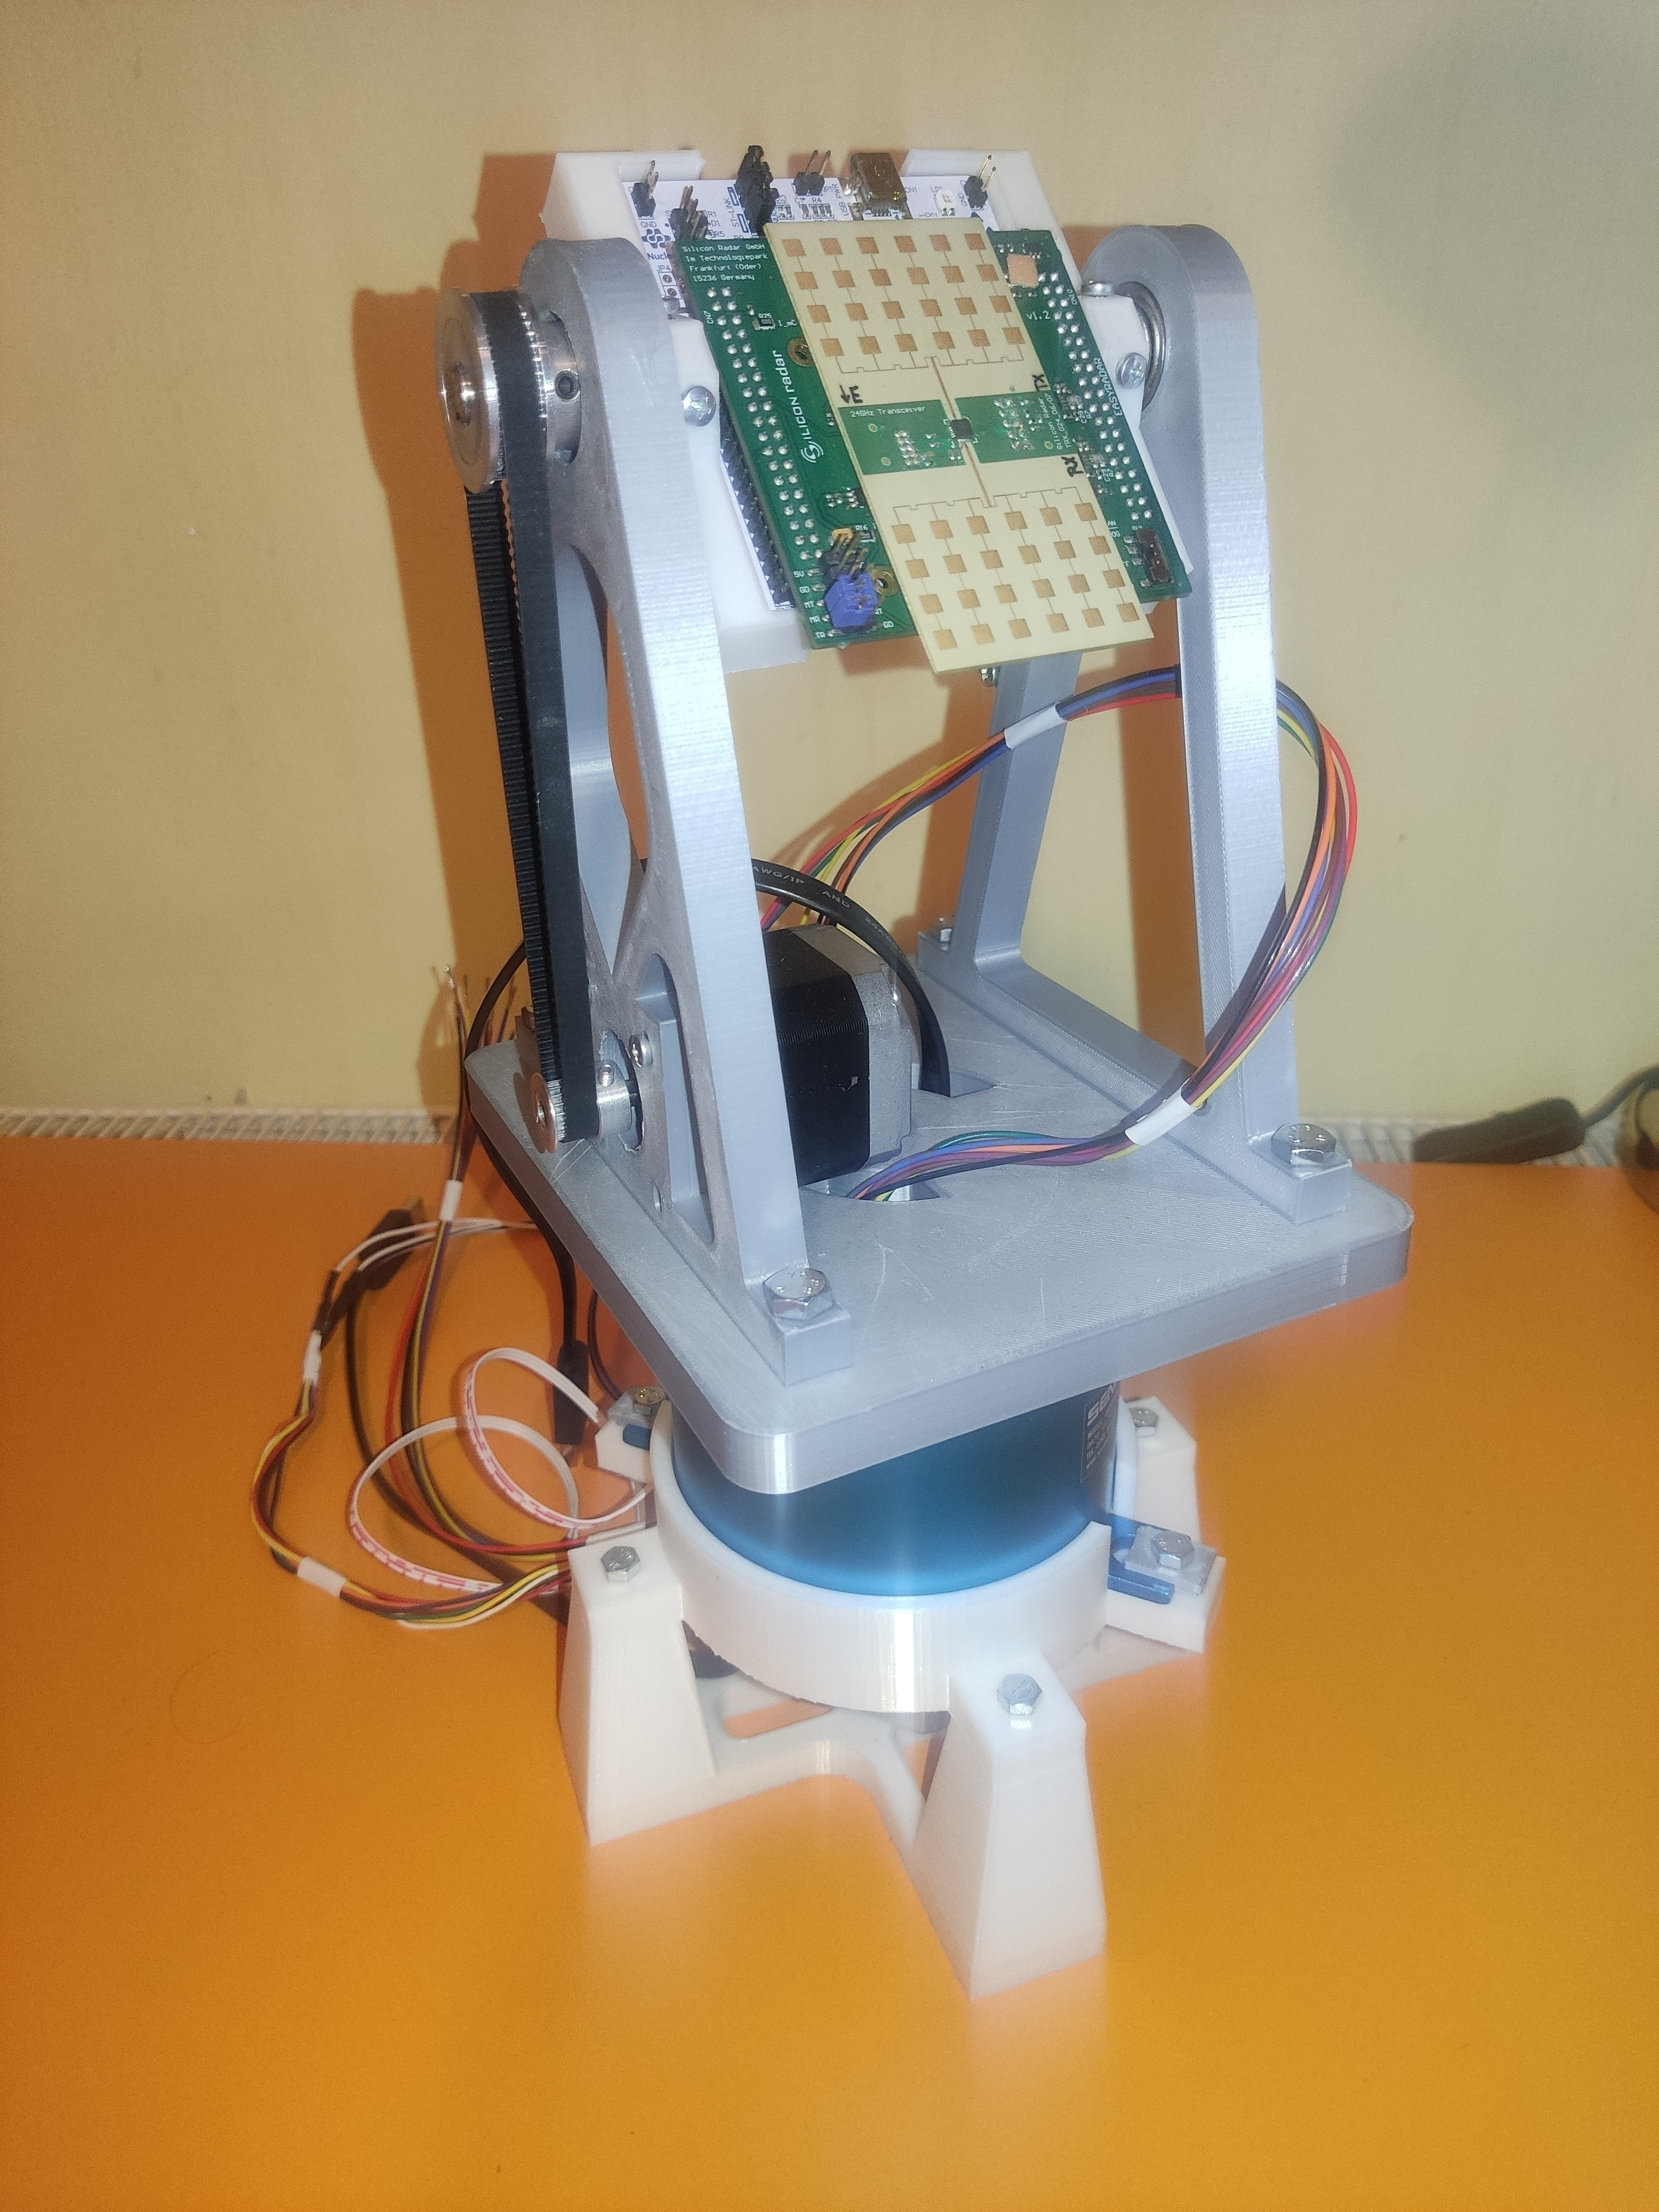
\includegraphics[width=0.75\textwidth]{../img/assembly_photo.jpg} % Replace with your image path
    \caption{Photo}
  \end{subfigure}
  \caption{Form of the final assembly}
  \label{fig:side_by_side}
\end{figure}

\section{Electronics}

Electronic side of the project is rather simple as we only need to control two stepper motors and have way to home them.
Whole system is controlled by ESP32 microcontroller since project doesn't require any special capabilities basic series of ESP32 microcontrollers is sufficient.

As the load on stepper motors is relatively low and whole platform will not be able to accumulate large amount of momentum simple stepper driver without feedback control is sufficient.
For this project A4988 stepper driver was chosen as it is cheap, easy to use and offers basic current control to smooth out stepper movement\cite{a4988}.

For homing  there were two prospective solutions -- Hall effect sensors, optical gates.
While Hall effect would offer sensing of any angle and thus be able to combat any drift in position during operation its integration would be rather complex.
As if orthogonal Hall effect sensors isn't placed exactly in axis of rotation calibration of the system is required\cite{hall}.
Thus for simplicity and ease of integration optical gates were chosen.


\chapter{Software realization}

In order to achieve maximal efficiency in processing commands and  maintain accurate driving of stepper motors workflow of the program is split into three distinct layers, as showed on diagram \ref{fig:code_diag}.
Using standard two component architecture with one part handling the parsing of commands and second managing their execution wasn't for this usecase - pre programming movements wouldn't be possible and precomputing multiple movements ahead unnecessary hard.
Now with increasing layer the amount of abstraction in command decreases and processing gets easier.
This enables the final stage to be really efficient thus moving form one command to another is more restricted by inertia of stepper motors.

\begin{figure}[h!]
  \centering


  \begin{tikzpicture}[scale=0.9, node distance=1.5cm]

    % Layer headers
    \node (comm_layer) [layerheader] at (0, 0) {Communication Layer};
    \node (app_layer) [layerheader] at (6, 0) {Application Layer};
    \node (hal_layer) [layerheader] at (12, 0) {HAL Layer};

    % Communication Layer
    \node (comm_start) [startstop, below of=comm_layer, yshift=-0.3cm] {Start};
    \node (wait_serial) [process, below of=comm_start] {Wait for serial data};
    \node (parse_gcode) [process, below of=wait_serial] {Parse G-code};
    \node (parse_success) [decision, below of=parse_gcode, align=center, yshift=-1.3cm] {Parsing\\ Successful?};
    \node (store_command) [process, below of=parse_success, align=center, yshift=-1.8cm] {Store command\\ queue ? program};
    \node (send_response) [process, below of=store_command,yshift=-0.25cm] {Send response};

    % Arrows in Communication Layer
    \draw [arrow] (comm_start) -- (wait_serial);
    \draw [arrow] (wait_serial) -- (parse_gcode);
    \draw [arrow] (parse_gcode) -- (parse_success);
    \draw [arrow] (parse_success.east) -- ++(1, 0) |- (send_response.east) node[midway, left, yshift=+0.25cm] {No};
    \draw [arrow] (parse_success.south) -- ++(0, -0.5) -| (store_command.north) node[midway, right, yshift=+0.05cm] {Yes};
    \draw [arrow] (store_command) -- (send_response);
    \draw [arrow] (send_response.west) -- ++(-0.5, 0) |- (wait_serial.west);

    % Application Layer
    \node (app_start) [startstop, below of=app_layer, yshift=-0.3cm] {Start};
    \node (update_position) [process, below of=app_start] {Update position};
    \node (check_queues) [decision, below of=update_position, yshift=-1.3cm] {Queues full?};
    \node (load) [process, below of=check_queues, align=center, yshift=-1.5cm] {Load command \\ queue ? program};
    \node (process_command) [process, below of=load,yshift=-0.25cm] {Process command};
    \node (store_command) [process, align=center, below of=process_command] {Add command \\ to stepper queue};

    % Arrows in Application Layer
    \draw [arrow] (app_start) -- (update_position);
    \draw [arrow] (update_position) -- (check_queues);
    \draw [arrow] (check_queues.east) -- ++(1, 0) |- (update_position.east) node[midway, left, xshift=0.2cm, yshift=+0.25cm,xshift=0.2cm] {Yes};
    \draw [arrow] (check_queues.south) -- ++(0, -0.5) -| (load.north) node[midway, right, yshift=+0.1cm] {No};
    \draw [arrow] (load.south) -- ++(0, -0.5) -- (process_command.north);
    \draw [arrow] (process_command) -- (store_command);
    \draw [arrow] (store_command.west) -- ++(-0.5, 0) |- (update_position.west);


    \node (hal_start) [startstop, below of=hal_layer, yshift=-0.3cm] {Start};
    \node (wait_queue) [process, below of=hal_start] {Wait on queue};
    \node (execute_command) [process, below of=wait_queue] {Execute command};
    \node (wait_command) [process, below of=execute_command] {Wait on command};
    \node (update_info) [process, align=center, below of=wait_command] {Update last \\command};

    % Arrows in HAL Layer
    \draw [arrow] (hal_start) -- (wait_queue);
    \draw [arrow] (wait_queue) -- (execute_command);
    \draw [arrow] (execute_command) -- (wait_command);
    \draw [arrow] (wait_command) -- (update_info);
    \draw [arrow] (update_info.west) -- ++(-0.5, 0) |- (wait_queue.west);

  \end{tikzpicture}

  \caption[Programm diagram]{Programm diagram}
  \label{fig:code_diag}
\end{figure}

\section{Communication layer}

Communication layer handles incoming data on serial line, reading from which is realized efficiently with the aid of RTOS queues.
Upon receiving data the text string is parsed and either push to queue (if we are declaring a programm) or added to programm declaration.

\section{Application layer}

Application layers does two main things - keeps track of current device position and schedules commands to be sent to steppers.
Tracking of current position and end position of last scheduled command also enables the application layer to do calculations needed for absolute positioning and limits enforcement.

One large change from normal G-code interpreters is the fact that if move command is issued only for a single axis second one is free to read next one and start executing it.
If this behavior is undesirable user needs to issue command to both axis - in relative positioning mode zero will result in no motion, in absolute positioning mode current position must be used.



\section{HAL Layer}

Final layer handles basic driving of steppers and provides Application layer with all necessary for position calculation.
In its loop we simply wait for a next command in the stepper queue.
If a command command is received programs set ups its execution and wait for the stepper or both steppers to finish moving after which its moves onto next command.
As all calculations regarding limits, positioning have been done beforehand in the application layer HAL layer can be really performant and efficient.

Main problem arises with generation of accurate PWM signal and having the ability to stop the generation upon given number of steps were taken.
From equation
%
\begin{equation}
  t_{\mathrm{delay}}(s) = \frac{60}{2\cdot N_{\mathrm{steps}} \cdot s},
  \label{eq:delay}
\end{equation}
%
where  $s$ is speed in RMP, $N_{\mathrm{steps}}$ number of steps of the stepper and  $t_{\mathrm{delay}}$ time between steps the time we can calculate that even for RPM of 30 delay between changes on output is 5ms on single stepper.
Take small microstepping of 2:1 into account and the thread would need to execute change every 2.5ms -- to fast to not arise problems with hardware watchdog.
Thus generating signal with purpose designed microcontroller peripherals is necessary.


ESP32 platform offers two solutions for this task - using Remote Controlled Transceiver (RMT) or Motor Control Pulse Width Modulation (MCPWM) combined with PCNT.
While RMT offers special capabilities like smoothly increasing PWM frequency it also brings many disadvantages: generating N number of pulses is available only only on the lastest version of ESP32 microcontrollers \cite{gitRMT}, synchronization can be only done cleanly with rather restrictive RMT specific API, there isn't a easy way to get information how far are we into move \cite{espRMT}.

For these reasons approach of combining MCPWM for pulse generation and PCNT for counting steps was chosen.
This allows for easy synchronization, realization of continous rotation and PCNT provides helpful API for counting steps\cite{espPCNT}.
Only disadvantage is strict limit of 15 bit counter making the maximal number of steps per move 32767.

\subsection{Performance of HAL Layer}


Table \ref{tab:performancepwm} shows stability of the PWM generation of the MCPWM module on different speeds.
Measurements were taken using Saleae Logic Pro 16 logic analyzer without any microstepping enabled.
We can clearly see that deviation in frequency is quite low thought the error increases with frequency and speed is consistently slightly faster than desired.
Still if we were to take 24000 steps with RPM of 120 relative error in time taken would be only $\epsilon = -0.004\%$


\begin{table}[h!]
  \centering
  \caption[Stability of PWM generation]{Stability of PWM generation}
  \begin{tabular}{| m{2cm} || m{2.5cm} | m{2.5cm} | m{2.5cm} | m{2.5cm} |}
    \hline
    RPM & $f_{\mathrm{desired}}$ (Hz) & $f_{\mathrm{low}}$ (Hz) & $f_{\mathrm{high}}$ (Hz) & $f_\mathrm{avg}$ (Hz) \\
    \hline
    10  & 33.334                      & 33.334                  & 33.334                   & 33.334                \\
    30  & 100                         & 100                     & 100.003                  & 100.002               \\
    60  & 200                         & 200                     & 200.01                   & 200.004               \\
    120 & 400                         & 400                     & 400.02                   & 400.007               \\
    \hline
  \end{tabular}
  \label{tab:performancepwm}
\end{table}

Attempt to measure how fast is switching between commands was done however as one can see from pictures
\ref{fig:switching}  the delay between commands isn't perceivable.
At least not on any reasonable RPM.
While the pictures is taken with transmission from step commands at 120 RPM to step command at 60 RPM measurements were also taken for different combinations of commands with similar results.

\begin{figure}[h!]
	\centering
	\includegraphics[width=0.7\textwidth]{../img/120rpm_to60_1.jpg}
	\includegraphics[width=0.7\textwidth]{../img/120rpm_to60_2.jpg}
	\caption[Moment of change between commands with 120RPM and 60RPM]{Moment of change between commands (120RPM $\Rightarrow$  60RPM)}
	\label{fig:switching}
\end{figure}

% RPM & desired  & low interval & high interval & deviation

% speed how fast follow on command gets executed

%% Table how fast are command processed
%% Table with how reliable is timing (with different rpm)

% vim.ft=tex
\chapter*{Conclusion}
\addcontentsline{toc}{chapter}{Conclusion}

Goal of this thesis was to realize a surveillance radar system based on FMCW technology.
This technology should enable accurate distance measurements of targets with a relatively low power consumption.
Instead of more conventional MIMO systems, a simpler solution was proposed with a single RX and TX antenna that relies on mechanical steering of the radar beam.

Using off-the-shelf components and 3D printed parts a custom rotary platform was designed and constructed.
All be it minor issues in regards to the belt tension on pitch axes in enables controlling of the radar position in both yaw and pitch directions.
Quality of life features such a automatic homing system or limits to the rotation were also implemented.
Whole system is controlled by an ESP32C6 microcontroller which interprets G-code like commands and drives the stepper motors.
Due to its similarities to other G-code base systems it should be readily adaptable to other systems.
In addition the platform was designed to support capabilities that aren't strictly necessary for the purpose of this thesis.

Capabilities of \sidar evaluation board were analyzed and were found to be suitable for the purpose of this thesis.
However not much room is left to improvement of the system as the board is limited by its low sampling rate and relatively slow microcontroller.
This limits the maximum detectable speed to tens of mm per second which effectively eliminates any possibility of tracking moving targets.
However it's ability to switch headers between 24~GHz and 122~GHz allows for a wide range of applications.

Control application for the system was developed in MATLAB.
This integrates both the rotary platform management and radar data processing.
Given rather generic design requirements of the application, larger degree of customization is allowed with simpler GUI menu.
The data processing pipeline is relatively standard reling on common techniques such as FFT, CFAR, DBSCAN and others.
Major downside is that configuration must be tailored to specific application and therefore the user must have a good understanding radar processing and some knowledge of the processing pipeline.
No predefined configurations for specific usecase are provided in the application.


FIX TODO

In addition whole processing is written in a way that if radar module was exchanged for a faster one capabilities could be much more extended without requring
keeping most of the codebase similar.
Aside from different function reading the data from the radar all code is relatively lightweight till the point position change is detected and multiple fft spectrums are being processed.

Thus radar with just increased chirp frequency would only lead to better speed recognition.
Especially if platform movement remained the same.
In case  of increase of platform rotation possible corrections would need to be done in the processing pipeline.

In case number of FFT points both in speed or range would be significantly larger that what has been tested (Maximal cube dimensions of around 500~MB were validated) different approach to cube update would be required.
First possibility would be leverages GPU acceleration to handle operations in the cube update.
Specifically the decaying of the cube would be possible for much larger dimensions.
In case of solely CPU based processing decay functions probably would be impractical for much larger cubes and the cube would need to be split into smaller chunks where only few ones would be loaded into RAM at one time -- depending on the current position of the platform and direction of travel.





\include{bibliography}
% \printbibliography

\listoffigures

\listoftables

\clearpage
\openright
\end{document}
